\problem{Positive Con Sequences}

%\begin{wrapfigure}{r}{0.5\linewidth}
%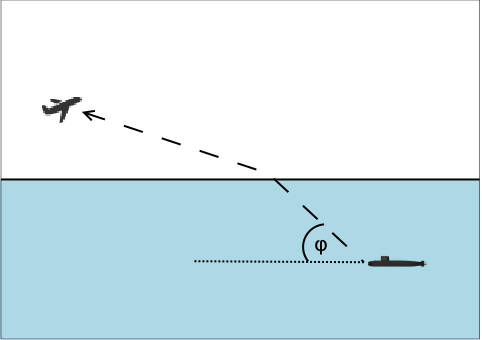
\includegraphics[width=\linewidth]{Refract/refract.png}
%\end{wrapfigure}

Your younger sister is studying for an upcoming standardized test in
mathematics, and needs practice with the common style of problem in
which the student is presented with a sequence of numbers with one
number missing and asked to fill in the missing value.

You are aware that the vast majority of these problems feature either
arithmetic sequences (where each number in the sequence is formed by
adding an integer constant to the prior number) or geometric sequences (where
each number in the sequence is formed by multiplying the prior number
by an integer constant).

Write a program that will help your sister drill on this style of
problem by allowing her to check her answers on sample problems.


\subsection*{Input}

Input will consist of one or more datasets.

Each dataset will be a single line containing $4$ integers defining a
sequence. One of these will be $-1$, denoting the missing value. The
remainder will be positive integers in the range $1\ldots \num{10000}$,
inclusive. Other than the $-1$ placeholder value, the values will be
in strictly increasing order.

End of input will be signaled by a line containing four $-1$
values.

\subsection*{Output}

For each dataset, print one line of output. 

If a positive integer in the range $1 \ldots \num{1000000}$ exists that
can be filled in to the missing value position to create an
arithmetic or geometric sequence, print that missing value. 

If there is no such positive integer, print -1.




\subsection*{Example}

Given the input:

\verbfile{Sequences/test0.in}


the output should be:

\verbfile{Sequences/test0.expected}



